


\chapter{Экспериментальная часть}\label{exp}
%\addcontentsline{toc}{chapter}{4 Экспериментальная часть}

Оценка качества работы алгоритмов. Экспериментальное сравнение работы различных алгоритмов нахождения среднего арифметического матрицы
(зависимость времени выполнения от размерности матриц).

\section{Технические характеристики}\label{texcharacters}

Технические характеристики устройства, на котором выполнялось тестирование:

\begin{enumerate}
    \item процессор: Intel® Core™ i3-7100U CPU @ 2.40GHz × 4; 
    \item память: 11,6 GiB;
    \item операционная система: Ubuntu 20.04.1 LTS.
\end{enumerate}

\section{Примеры работы}\label{examples}

На рисунках \ref{ris:w1}, \ref{ris:w2}, \ref{ris:w3} показаны примеры работы.

\begin{figure}[H]
    \center{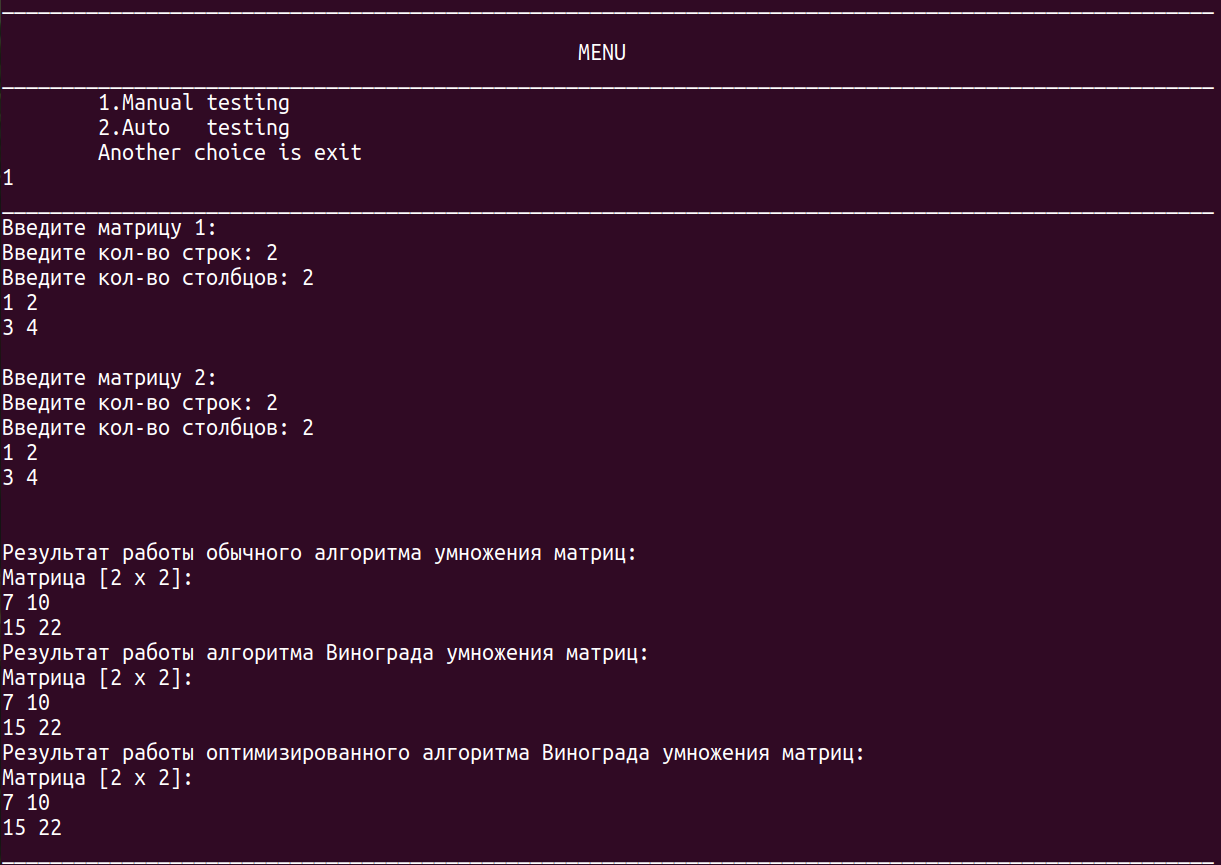
\includegraphics[scale=0.35]{w2}}
    \caption{Пример 1}
    \label{ris:w1}
\end{figure}
  
\begin{figure}[H]
    \center{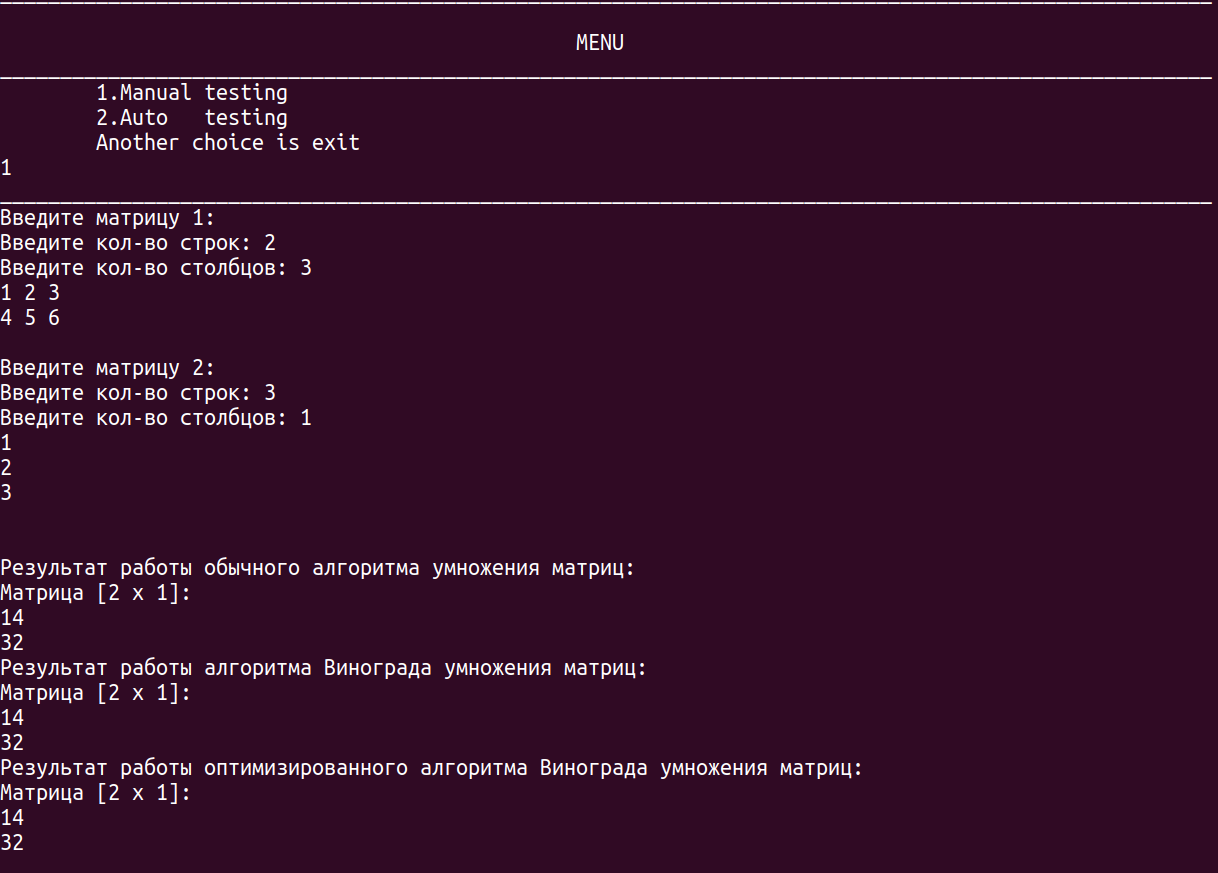
\includegraphics[scale=0.35]{w3}}
    \caption{Пример 2}
    \label{ris:w2}
\end{figure}
  
%\begin{figure}[H]
%    \center{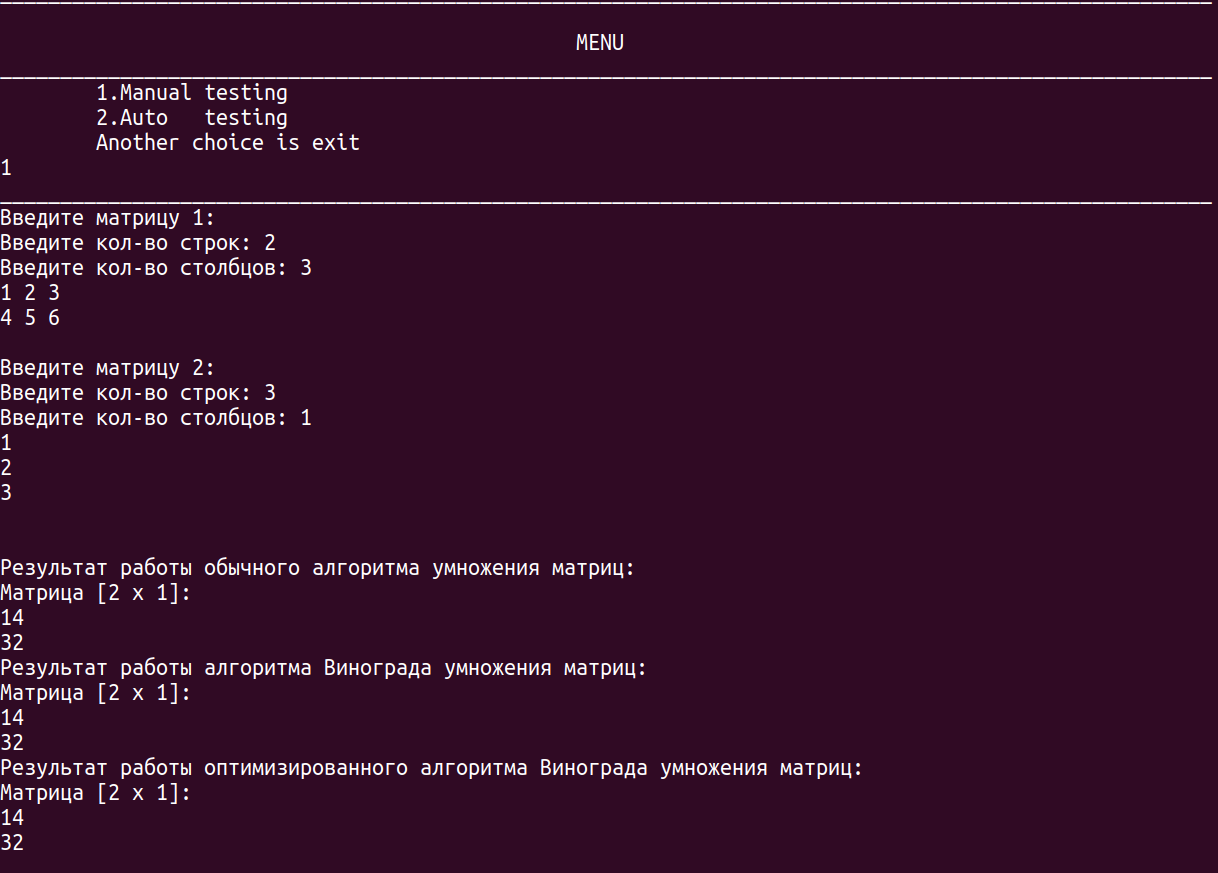
\includegraphics[scale=0.35]{w3}}
%    \caption{Ручное тестирование: тест 3}
%    \label{ris:w4}
%\end{figure}
  
\begin{figure}[H]
    \center{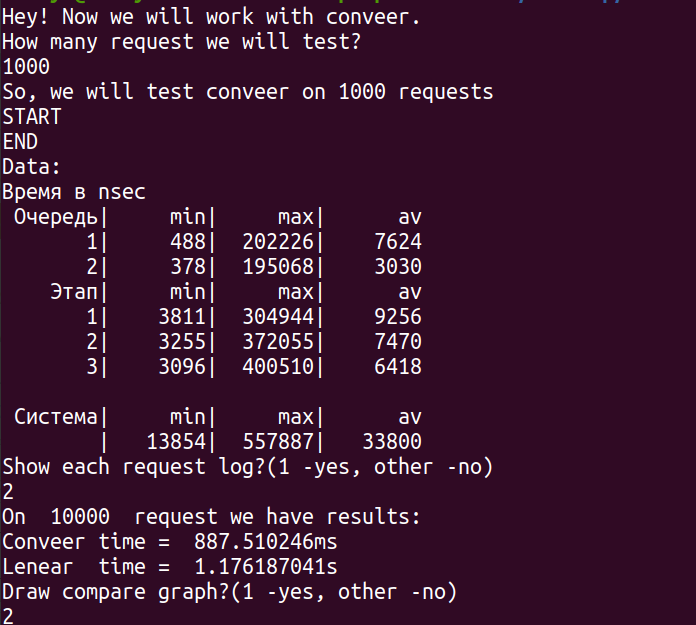
\includegraphics[scale=0.25]{w1}}
    \caption{Пример 3}
    \label{ris:w3}
\end{figure}

\section{Замеры времени}\label{experimentgraph}

Таблица \ref{tab:resulttime} содержит резульаты замеров времени при 1, 2, 4, 8, 16, 32 потоках
\begin{table}[ht]
    \caption{Замеры времени (в $10^{-2}$сек)}
    \centering
    \scriptsize
\begin{tabular}{ l | l | l | l | l | l | l | l | l | l | l | l |l |l  }
Длина&     stand&1     стр.&1    стол.&2     стр.&2    стол.&4     стр.&4    стол.&8     стр.&8    стол.&16    стр.&16   стол.&32    стр.&32   стол. \\ \hline
100&  0.0079&  0.0067&  0.0065&  0.0064&  0.0064&  0.0087&  0.0088&  0.0196&  0.0198&  0.0412&  0.0443&  0.0839&  0.0855\\
200&  0.0168&  0.0199&  0.0194&  0.0126&  0.0126&  0.0138&  0.0133&  0.0239&  0.0249&  0.0447&  0.0467&  0.0898&  0.0914\\
300&  0.0358&  0.0414&  0.0411&  0.0232&  0.0228&  0.0207&  0.0252&  0.0332&  0.0383&  0.0495&  0.0507&  0.0946&  0.1039\\
400&  0.0639&  0.0693&  0.0719&  0.0364&  0.0376&  0.0319&  0.0351&  0.0558&  0.0645&  0.0577&  0.0771&  0.1022&  0.1075\\
500&  0.0997&  0.1057&  0.1052&  0.0543&  0.0544&  0.0459&  0.0518&  0.0760&  0.0920&  0.0738&  0.1063&  0.0999&  0.1463\\
600&  0.1441&  0.1504&  0.1496&  0.0777&  0.0792&  0.0626&  0.0685&  0.1003&  0.1317&  0.0893&  0.1630&  0.1138&  0.2116\\
700&  0.1963&  0.2028&  0.2017&  0.1045&  0.1073&  0.0840&  0.0927&  0.1293&  0.1749&  0.1198&  0.2155&  0.1382&  0.2990\\
800&  0.2572&  0.2636&  0.2618&  0.1334&  0.1403&  0.1135&  0.1197&  0.1735&  0.2156&  0.1383&  0.2923&  0.1621&  0.4061\\
900&  0.3254&  0.3320&  0.3301&  0.1698&  0.1783&  0.1297&  0.1509&  0.1992&  0.2516&  0.1661&  0.3670&  0.1910&  0.5182\\
1000&  0.4030&  0.4085&  0.4085&  0.2068&  0.2152&  0.1608&  0.1856&  0.2247&  0.3022&  0.2117&  0.4611&  0.2243&  0.6299\\
\end{tabular}
\label{tab:resulttime}
\end{table}



На рисунках \ref{ris:graph1} и \ref{ris:graph2} показаны графические результаты сравнения исследуемых алгоритмов по времени. 

\begin{figure}[H]
    \center{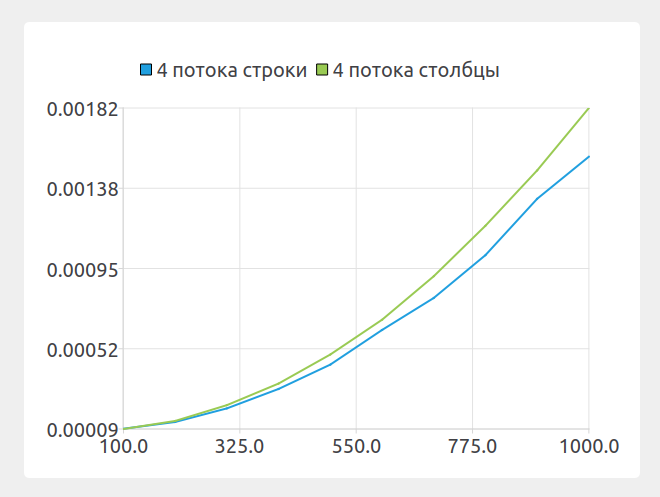
\includegraphics[scale=0.45]{graph3}}
    \caption{Сравнение распараллеленого по строкам и столбцам алгоритмов}
    \label{ris:graph2}
\end{figure}

\begin{figure}[H]
    \center{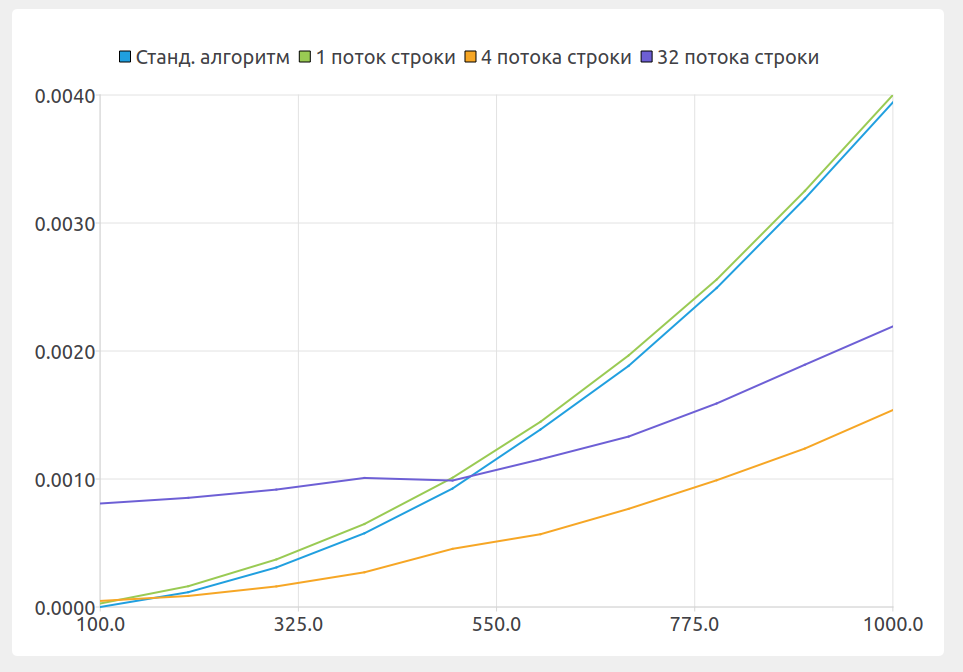
\includegraphics[scale=0.4]{graph5}}
    \caption{Сравнение стандартного и распараллеленых по строкам алгоритмов}
    \label{ris:graph1}
\end{figure}

\section{Сравнительный анализ алгоритмов}\label{comparepart}

По результатам экспериментов можно заключить следующее:
\begin{enumerate}
    \item при относительно небольшом размере матриц (менее 100x100) использование потоков для уменьшения времени исполнения 
    нецелесообразно, так как накладные расходы времени на управление потоками и mutexами больше, чем выигрыш от параллельного выполнения 
    выполнения вычислений;
    \item использование по крайней мере двух потоков даёт ощутимый выигрыш по времени по сравнению с однопоточной версией алгоритма; 
    \item использование одного потока в многопоточных версиях алгоритма проигрывает по времени по сравнению с однопоточной версией 
    алгоритма, что объясняется накладными расходами времени на управление потоками и mutex-ами;
    \item использование 8 и 32 потоков показывает результат по времени несколько хуже, чем при 4 потоках, из чего следует, 
    что увеличение потоков даёт выигрыш по времени лишь до достижения определённого количества, так как появляются большие накладные 
    затраты по времени для управления большим количеством потоков и mutex-ов;
    \item параллельные версии алгоритма выполняются за приблизительно одинаковое время при одном потоке. Однако, использование большего 
    количества потоков выявляет, что многопоточность по строкам быстрее многопоточности по столбцам;
    \item наиболее быстродейственно алгоритм действует на 4 потоках, что равно количеству логических процессоров на испытуемом компьютере/
\end{enumerate}

\section{Вывод экспериментальной части}\label{experimentresult}

Таким образом, в задачах, где выполняются несколько действий параллельно и независят от результатов 
предыдущих действий, выгодно использовать потоки. Оптимальным количеством потоков является число равное кол-ву 
процессоров на испытуемом компьютере.

\addcontentsline{toc}{chapter}{{Заключение}}
\chapter*{Заключение}\label{exit}

В данной работе были изучены алгоритмы нахождения среднего арифметического матрицы. 
Получены практические навыки реализации параллельных алгоритмов. 
Проведён сравнительный анализ алгоритмов по времени. 
Экспериментально подтверждены различия в эффективности алгоритмов с указанием лучших и худших случаев. 
Цель работы достигнута, решены поставленные задачи. 
